\documentclass[]{article}
\usepackage{lmodern}
\usepackage{amssymb,amsmath}
\usepackage{ifxetex,ifluatex}
\usepackage{fixltx2e} % provides \textsubscript
\ifnum 0\ifxetex 1\fi\ifluatex 1\fi=0 % if pdftex
  \usepackage[T1]{fontenc}
  \usepackage[utf8]{inputenc}
\else % if luatex or xelatex
  \ifxetex
    \usepackage{mathspec}
  \else
    \usepackage{fontspec}
  \fi
  \defaultfontfeatures{Ligatures=TeX,Scale=MatchLowercase}
\fi
% use upquote if available, for straight quotes in verbatim environments
\IfFileExists{upquote.sty}{\usepackage{upquote}}{}
% use microtype if available
\IfFileExists{microtype.sty}{%
\usepackage[]{microtype}
\UseMicrotypeSet[protrusion]{basicmath} % disable protrusion for tt fonts
}{}
\PassOptionsToPackage{hyphens}{url} % url is loaded by hyperref
\usepackage[unicode=true]{hyperref}
\hypersetup{
            pdfborder={0 0 0},
            breaklinks=true}
\urlstyle{same}  % don't use monospace font for urls
\usepackage[margin=1in]{geometry}
\usepackage{graphicx,grffile}
\makeatletter
\def\maxwidth{\ifdim\Gin@nat@width>\linewidth\linewidth\else\Gin@nat@width\fi}
\def\maxheight{\ifdim\Gin@nat@height>\textheight\textheight\else\Gin@nat@height\fi}
\makeatother
% Scale images if necessary, so that they will not overflow the page
% margins by default, and it is still possible to overwrite the defaults
% using explicit options in \includegraphics[width, height, ...]{}
\setkeys{Gin}{width=\maxwidth,height=\maxheight,keepaspectratio}
\IfFileExists{parskip.sty}{%
\usepackage{parskip}
}{% else
\setlength{\parindent}{0pt}
\setlength{\parskip}{6pt plus 2pt minus 1pt}
}
\setlength{\emergencystretch}{3em}  % prevent overfull lines
\providecommand{\tightlist}{%
  \setlength{\itemsep}{0pt}\setlength{\parskip}{0pt}}
\setcounter{secnumdepth}{0}
% Redefines (sub)paragraphs to behave more like sections
\ifx\paragraph\undefined\else
\let\oldparagraph\paragraph
\renewcommand{\paragraph}[1]{\oldparagraph{#1}\mbox{}}
\fi
\ifx\subparagraph\undefined\else
\let\oldsubparagraph\subparagraph
\renewcommand{\subparagraph}[1]{\oldsubparagraph{#1}\mbox{}}
\fi

% set default figure placement to htbp
\makeatletter
\def\fps@figure{htbp}
\makeatother

\usepackage{multirow} \usepackage{multicol} \usepackage{amssymb} \usepackage{hyperref} \usepackage{booktabs} \hypersetup{ colorlinks=true, linkcolor=blue, filecolor=magenta, urlcolor=cyan}

\author{}
\date{\vspace{-2.5em}}

\begin{document}

\newpage

\begin{flushright}
    \textbf{Équipe 8}
\end{flushright}

\begin{center}
    \vspace{2\baselineskip}
    Charles Comeau \\
    (111 185 421) \\ \vspace{1\baselineskip} Nicholas Langevin \\
    (111 184 631) \\
    \vspace{1\baselineskip}
    Andréanne Larouche \\
    (111 190 518) \\
    \vspace{7\baselineskip}
    Apprentissage statistique en actuariat\\
    ACT-3114 \\
    \vspace{7\baselineskip}
    {\large
    \textbf{Analyse des données de renouvellement d'assurance}} \\
    \vspace{8\baselineskip}
    présenté à \\
    Marie-Pier Côté \\
    \vspace{9\baselineskip}
    École d’actuariat \\
    Université Laval \\
    27 février 2020
\end{center}

\newpage

\tableofcontents

\newpage

\section{Introduction}\label{introduction}

Les contrats d'assurance IARD sont pour la plupart d'une durée d'un an;
conséquemment, le renouvellement des polices est une étape répétitive
pour les assureurs. Il est important pour ceux-ci de bien prévoir
combien d'assurés resteront avec eux pour la prochaine année. Ces
prévisions peuvent avoir de l'importance sur les stratégies de
renouvellement, entre autres, puisque plus un assuré à des chances de
renouveler, plus l'assureur voudra lui charger plus cher pour augmenter
sont profit. D'un autre côté, cette prévision peut aussi être utilisée
dans les stratégies nouvelles affaires puisque si beaucoup d'assurés
résignent leur police, la croissance en unité sera affectée et celle-ci
pourra prévoir des rabais pour les nouvelles assurées dans le but de
compenser.

Notre travail se concentre sur la modélisation et la prédiction de la
probabilité de non-renouvellement des assurés. Pour ce faire, nous avons
utilisé un jeu de données, nommées \emph{eudirectlapse}, provenant du
paquetage \emph{CASdataset} (Dutang and Charpentier (2019)). Ce jeu de
données représente les primes de \(23 060\) polices avant et après le
renouvellement ainsi que leurs statuts de renouvellement ou de
résignation. La base de données comprend aussi d'autres variables qui
caractérisent chaque contrat comme l'âge des conducteurs, le type de
conducteur, etc. Finalement, cette base de données provient d'un
assureur inconnu et pour une année inconnue.

Finalement, dans le but de comparer correctement les modèles utilisés,
20\% de la base de données a été mis de côté pour servir comme données
de test. Puisque les données sont déséquilibrées, la proportion de
résignation a été conservée autant dans les données d'entrainement que
de tests.

\newpage

\section{Modèle de base}\label{moduxe8le-de-base}

Pour le modèle de base, nous utiliserons un modèle linéaire généralisé
avec une distribution binomiale. Plus précisément, il s'agit d'une
distribution binomiale avec \(m = 1\) donc une distribution Bernouilli.
La valeur de y est de 1 lorsque l'assuré résigne et de 0 lorsqu'il
renouvèle. On s'intéresse à modéliser la probabilité que l'assuré ne
renouvelle pas son contrat. Pour ce faire, le lien logistique sera
utilisé pour faire le lien entre la probabilité et le prédicteur
linéaire. Ainsi nous avons :

\begin{align}
    \ln \frac{\pi_{res}}{1 - \pi_{res}} = \beta_0 + \sum_{i=1}^p \beta_i x_i,
\end{align}

où nous voulons maximiser la vraisemblance d'une bernouilli. Ainsi les
valeurs des paramètres sont obtenues en maximisant l'équation suivante.

\begin{align}
    \max\limits_{(\beta_0, \beta_j)} exp\left\{ \sum_{i=1}^n \left( y_{i} (\beta_{0} + \sum_{j=1}^p \beta_{j} x_{j} ) - ln \left(1 + e^{\beta_{0} + \sum\limits_{j=1}^p \beta_{j} x_{j}} \right)\right) \right\}
\end{align}

Pour ce modèle de base, il n'a pas d'optimisation à faire pour les
hyperparamètres. Par contre, il est pertinent d'effectuer une sélection
des variables explicatives pour rendre le modèle moins complexe. Nous
avons effectué des tests du rapport de vraisemblance pour la sélection
des variables. Un niveau de confiance de 99\% a été choisi pour ces
tests. Au final, il y a 7 variables parmi les 19 qui ne sont \textbf{pas
sélectionnées} pour le modèle de base les voici:

\begin{multicols}{2}
\begin{itemize}
\item policy\_caruse
\item policy\_nbcontract
\item prem\_pure
\item prem\_index
\end{itemize}
\columnbreak
\begin{itemize}
\item vehicl\_agepurchase
\item vehicl\_powerkw
\item vehicl\_garage
\end{itemize}
\end{multicols}

C'est donc de dire que ces variables ne seront pas considérées pour les
prévisions avec le modèle de base. Le modèle retourne comme prévision
une probabilité que le client ne renouvelle pas son contrat. Il est donc
nécessaire de déterminer un seuil minimal pour lequel l'observation aura
une prévision correspondant à une résignation et si la prévision est
inférieure à ce seuil alors la prévision est un renouvellement. Il a été
décidé d'utiliser le seuil optimal de la courbe ROC sur les données
d'entrainement. C'est le seuil pour lequel le point sur la courbe ROC se
retrouve le plus proche du coin supérieur gauche du graphique. Ce seuil
est optimal pour un compromis entre les statistiques de sensitivité, le
taux de bonne classification des résignations, et de spécificité, le
taux de bonne classification des renouvellements. Voici le tableau de
confusion obtenu des données d'entrainement ainsi que des statistiques
d'intérêt.

\begin{table}[!htb]
\centering
\begin{minipage}{0.48\linewidth}
\begin{tabular}{c|cc} 
\multicolumn{1}{c}{} & \multicolumn{2}{c}{Prédictions} \\
Observations & Renouvellement & Résignation \\
\hline Renouvellement & 9243 & 6842 \\
Résignation & 896 & 1468 \\
\hline
\end{tabular}
\end{minipage}
\hfill
\begin{minipage}{0.48\linewidth}
\centering
\begin{tabular}{c|c} 
Statistiques & \% \\
\hline
Seuil optimal & 12.522  \\
Sensitivité & 62.098 \\
Spécificité & 57.463 \\
\hline
\end{tabular}
\end{minipage}
\end{table}

Les statistiques de sensitivité et de spécificité avoisinent toutes les
deux les 60\% dans le cas où nous prenons le seuil optimal. Cela veut
dire que le modèle de base classifie avec un taux similaire les
résignations et les renouvellements. Par contre on constate qu'en
procédant ainsi, il y a un grand nombre de clients pour lesquels le
modèle de base prédit une résignation alors qu'en fait ce sont des
clients enclins à renouveler. Il sera intéressant de voir si les autres
modèles amélioreront cet aspect. Une comparaison avec les autres modèles
sera établie avec l'échantillon test plus loin dans le rapport.

\newpage

\section{Ajustement des modèles}\label{ajustement-des-moduxe8les}

\subsection{Modèle linéaire généralisé avec régularisation
Lasso}\label{moduxe8le-linuxe9aire-guxe9nuxe9ralisuxe9-avec-ruxe9gularisation-lasso}

Comme dans le cas d'un modèle généralisé (\emph{GLM}), la distribution
binomiale a été choisie pour modéliser la probabilité de résignation. De
plus, le lien \emph{logistique} a été utilisé. Si \(\pi_{res}\)
représente la probabilité que l'assuré résigne sont contrat, alors le
modèle peut être écrit comme

\begin{align}
    \ln \frac{\pi_{res}}{1 - \pi_{res}} = \beta_0 + \sum_{i=1}^p \beta_i x_i,
\end{align}

où les \((\beta_0, \beta_j)\) sont obtenue en minimisant l'équation
suivant

\begin{align}
    \min\limits_{(\beta_0, \beta_j)} -\left[\frac{1}{N}\sum_{i=1}^n 
    y_i (\beta_0 + \sum_{i=1}^p \beta_i x_i) + 
    \log( 1 + e^{(\beta_0 + \sum_{i=1}^p \beta_i x_i)}) \right]
    + \lambda \sum_{j=1}^p |\beta_j|.
\end{align}

La fonction de minimisation comprend le paramètre \(\lambda\) qui doit
être déterminé d'avance. La valeur optimale a été choisie par validation
croisée à \(10\) plis. La \autoref{fig:lasso.valid} montre le résultat
pour deux métriques différentes, soit la \emph{deviance} de la loi
binomiale et l' \emph{AUC}. Les deux valeurs optimales pour \(\lambda\)
sont 0.000682 et 0.0003556 respectivement.

\begin{figure}
\centering
\begin{minipage}{0.48\linewidth}

\begin{center}\includegraphics{Rapport_Final_files/figure-latex/lasso.plotBestLambda.dev-1} \end{center}
\end{minipage}
\hfill
\begin{minipage}{0.48\linewidth}

\begin{center}\includegraphics{Rapport_Final_files/figure-latex/lasso.plotBestLambda.auc-1} \end{center}
\end{minipage}
\caption{Résultats de la validation croisée à $10$ plis selon différentes
métriques pour déterminer le $\lambda$ optimal. Les valeurs optimales obtenues
sont de 
0.000682 pour la 
\emph{deviance} d'une binomial et de
0.0003556 pour 
\emph{AUC}.}
\label{fig:lasso.valid}
\end{figure}

Selon la valeur optimale de \(\lambda\) qui optimise chacune des
métriques, les variables qui voient leurs coefficients (\(\beta\))
rétrécir à \(0\) sont similaires. Ces variables sont listées dans le
\autoref{tbl:lasso.variable0}. Il est intéressant de voir que les
variables \emph{prem\_pure} et \emph{prem\_last} ne semblent pas
importantes, ce qui confirme l'hypothèse du premier rapport où la prime
absolue n'est pas importante. C'est pourquoi initialement la variable
\emph{prem\_index = prem.final / prem\_last} avait été crée. Nous
verrons plus tard que cette dernière est importante dans le modèle
d'arbre. Finalement, il est pertinent de mentionner que c'est la
variable représentant la prime pure qui est exclue du modèle et non la
variable contenant la prime finale chargée au client, qui inclut
probablement des rabais/surcharge en fonction du marché. Conséquemment,
ceci montre que les caractéristiques du marché impactent la probabilité
de non-renouvellement, ce qui est logique puisqu'il est normal que le
taux de rétention d'un assureur soit impacté par sa compétitivité dans
le marché.

\begin{table}[ht]
\centering
\caption{Variables qui voient leur coeficient rétricire à $0$ (noté
          par un x). La colonne \emph{deviance} représente les variables
          exclut par le $\lambda$ optimal selon cette métrique et pareillement
          pour la colonne \emph{AUC}.} 
\label{tbl:lasso.variable0}
\begin{tabular}{cccc}
  \hline
Variable & Niveau & Deviance & AUC \\ 
  \hline
policy caruse & private or freelance work & x & x \\ 
  prem last & - & x & x \\ 
  prem pure & - & x & x \\ 
  vehicl garage & street & x &   \\ 
  vehicl region & Region 03 & x & x \\ 
  vehicl region & Region 08 & x & x \\ 
  vehicl region & Region 10 & x &   \\ 
   \hline
\end{tabular}
\end{table}

Pour déterminer si une prédiction est à résignation ou à renouvellement,
il faut déterminer le seuil optimal qui maximise la sensitivité et la
spécificité. Celui-ci a été sélectionné selon le critère suivant

\begin{align}
    \min\{ (1-\text{sentitivité})^2 + (1-\text{spécificité})^2 \}.
\end{align}

Ce critère représente le point le plus proche du coin haut gauche de la
courbe ROC. Puisque les 2 modèles ont des courbes ROC similaires, le
seuil optimal est aussi similaire. Le \autoref{tbl:lasso.confMatrix}
montre les tableaux de confusion résultants. Dans le cas du modèle
utilisant la \emph{deviance}, la sensitivité est de 0.60339 et la
spécificité est de 0.48371. Dans le modèle utilisant l' \emph{AUC}, la
sensitivité est de 0.60339 et la spécificité est de 0.60339. On remarque
que l'erreur la plus fréquente dans les deux cas est de prédire
faussement résignation. Ceci pourrait causé des erreurs de
rentabilisation au renouvellement puisque la compagnie ne passerait pas
de grandes augmentations de prime à ces clients par \textbf{fausse} peur
que ceux-ci résigne leur contrat.

\begin{table}[!hb]
\centering
\caption{Tableau de confusion en utilisant le seuil optimal pour les deux 
différent modèle.}
\label{tbl:lasso.confMatrix}
\begin{minipage}{0.48\linewidth}
\begin{tabular}{l|cc}
\multicolumn{1}{c}{} & \multicolumn{2}{c}{Prédiction} \\
Deviance: & Renouvellement & Résignation \\
\hline
Renouvellement & 8340 & 7745 \\
Résignation    & 1311 & 1053 \\
\hline
\end{tabular}
\end{minipage}
\hfill
\begin{minipage}{0.48\linewidth}
\begin{tabular}{l|cc}
\multicolumn{1}{c}{} & \multicolumn{2}{c}{Prédiction} \\
AUC: & Renouvellement & Résignation \\
\hline
Renouvellement & 8296 & 7789 \\
Résignation    & 1306 & 1058 \\
\hline
\end{tabular}
\end{minipage}
\end{table}

\newpage

\subsection{k plus proches voisins}\label{k-plus-proches-voisins}

Le modèle des \emph{k} plus proches voisins calcule les prédictions en
utilisant la distance euclidienne, ce qui veut dire que les variables
catégorielles non ordonnées doivent être transformées en \((c-1)\)
variables binaires. Aussi, les variables catégorielles ordonnées ont été
transformées en des variables numériques disctrètes \((1, 2, 3,...)\).
Le modèle des \emph{k} plus proches voisins comprend un seul
hyperparamètre, soit le nombre de voisins (\emph{k}) à utiliser pour la
prédiction. Ce choix a été optimisé en utilisant une validation croisée
à 4 plis. La valeur de \emph{k} qui maximise l'aire sous la courbe ROC
est de 240. Ces valeurs, pour chaque valeur de \emph{k}, sont présentées
dans la \autoref{tbl:knn.plot-bestTune}.

\begin{figure}

{\centering \includegraphics{Rapport_Final_files/figure-latex/knn.plot_bestTune-1} 

}

\caption{\label{tbl:knn.plot-bestTune} Valeurs de l'aire sous la courbe ROC en fonction de différentes valeurs de \emph{k}}\label{fig:knn.plot_bestTune}
\end{figure}

Les prédictions pour les données test qui serviront à comparer les
modèles seront classifiées en fonction de la classe majoritaire des 240
observations les plus proches. Puisque nous avons des données
déséquilibrées, ce type de modèle pourrait avoir des prévisions
médiocres puisqu'il va être rare plus de 50\% soit des résignations dans
les plus proches voisins.

\newpage

\subsection{Arbre de classification}\label{arbre-de-classification}

Le modèle d'arbre de classification offre la possibilité d'utiliser deux
fonctions de perte différence. Si \emph{K} représente le nombre de
classes, alors un premier choix comme fonction de perte peut être l'
\emph{indice de Gini}, défini comme

\begin{align}
    \mathcal{L}_G = \sum_{k=1}^K \widehat{P}_{mk} (1 - \widehat{P}_{mk}).
\end{align}

Dans un deuxième cas, il est possible d'utiliser la \emph{deviance}
négative d'une loi bernoulli (ou encore l'\emph{entropie croisée})
defini comme

\begin{align}
    \mathcal{L}_D = \sum_{k=1}^K \widehat{P}_{mk} \ln( \widehat{P}_{mk}).
\end{align}

La procédure d'optimisation des hyperparamètres a été effectuée pour
chacune des deux fonctions de perte. En premier lieu, un arbre complet
\(T_0\) a été entrainé par validation croisée en 10 plis. Celui-ci est
défini comme un arbre construit avec un paramètre de complexité
(\emph{cp}) à 0 ainsi qu'un nombre minimal d'observations dans chaque
feuille (\emph{minbucket}) à 1. La \autoref{fig:tree.plotArbreT0}
présente l'erreur obtenue par validation croisée pour certaines valeurs
de \emph{cp}. Selon cette métrique, le meilleur modèle serait l'arbre
racine, ce qui signifie que la prédiction serait la même pour toutes les
données. La métrique \emph{AUC} sera considérée par la suite pour
l'optimisation des hyperparamètres.

\begin{figure}

{\centering \includegraphics{Rapport_Final_files/figure-latex/tree.plotArbreT0-1} 

}

\caption{Résultats de la validation croisée pour un arbre complet $T_0$ utilisant \emph{Gini} comme fonction de perte.}\label{fig:tree.plotArbreT0}
\end{figure}

\newpage

Pour la suite, l'optimisation du \emph{cp} a été effectuée sur plusieurs
valeurs de \emph{minbucket}. La \autoref{tbl:tree.auc} montre les
résultats de l'aire sous la courbe ROC (\emph{AUC}) pour différente
valeur de \emph{minbucket} en fonction du \emph{cp} optimal. À droite,
la fonction de perte utilisée est l' \emph{indice de Gini}, alors qu'à
gauche, la fonction de perte utilisée est l' \emph{entropie croisée}.
Ces valeurs ont été obtenues par validation croisée à 4 plis.

\begin{table}[!ht]
\caption{\emph{AUC} pour différentes valeurs de \emph{minbucket} en fonction du 
\emph{cp} optimal. À gauche, la fonction de perte utilisée est l'indice de 
\emph{Gini} et à droite l'\emph{entropie croisée}.}
\label{tbl:tree.auc}
\begin{minipage}{0.48\linewidth}
\centering
\begin{tabular}{ccc}
\hline
\multicolumn{3}{c}{Indice de Gini} \\
minbucket & cp & ROC \\ 
  \hline
10 & 0.000331 & 0.584 \\ 
  11 & 0.000229 & 0.584 \\ 
  12 & 0.000076 & 0.586 \\ 
  13 & 0.000204 & 0.582 \\ 
  14 & 0.000025 & 0.586 \\ 
  15 & 0.000051 & 0.584 \\ 
   \hline
16 & 0.000178 & 0.588 \\ 
   \hline
17 & 0.000025 & 0.579 \\ 
  18 & 0.000076 & 0.580 \\ 
  19 & 0.000127 & 0.583 \\ 
  20 & 0.000051 & 0.575 \\ 
   \hline
\end{tabular}
\end{minipage}
\hfill
\begin{minipage}{0.48\linewidth}
\centering
\begin{tabular}{ccc}
\hline
\multicolumn{3}{c}{Entropie croisée} \\
minbucket & cp & ROC \\ 
  \hline
10 & 0.000178 & 0.571 \\ 
  11 & 0.000204 & 0.583 \\ 
  12 & 0.000204 & 0.583 \\ 
  13 & 0.000076 & 0.583 \\ 
  14 & 0.000051 & 0.583 \\ 
   \hline
15 & 0.000076 & 0.588 \\ 
   \hline
16 & 0.000204 & 0.573 \\ 
  17 & 0.000051 & 0.579 \\ 
  18 & 0.000407 & 0.571 \\ 
  19 & 0.000051 & 0.588 \\ 
  20 & 0.000076 & 0.577 \\ 
   \hline
\end{tabular}
\end{minipage}
\end{table}

Les résultats, peut importe la fonction de perte utilisée, sont
similaires dans pour l'hyperparamètre \emph{minbucket}. Par contre, le
modèle utilisant l'\emph{indice de Gini} est optimal pour une valeur de
\emph{cp} plus élevée, résultant en un arbre moins complexe. Il est donc
préférable de prendre ce modèle puisqu'il risque potentiellement de
moins faire de surapprentissage sur les données d'apprentissage. Ainsi,
le modèle choisi utilisira un \emph{cp} de 0.00017811, un
\emph{minbucket} de 16 et utilisera l' \emph{indice de Gini} comme
fonction de perte. La figure \autoref{fig:arbre} illustre l'arbre
résultant.

\begin{figure}

{\centering 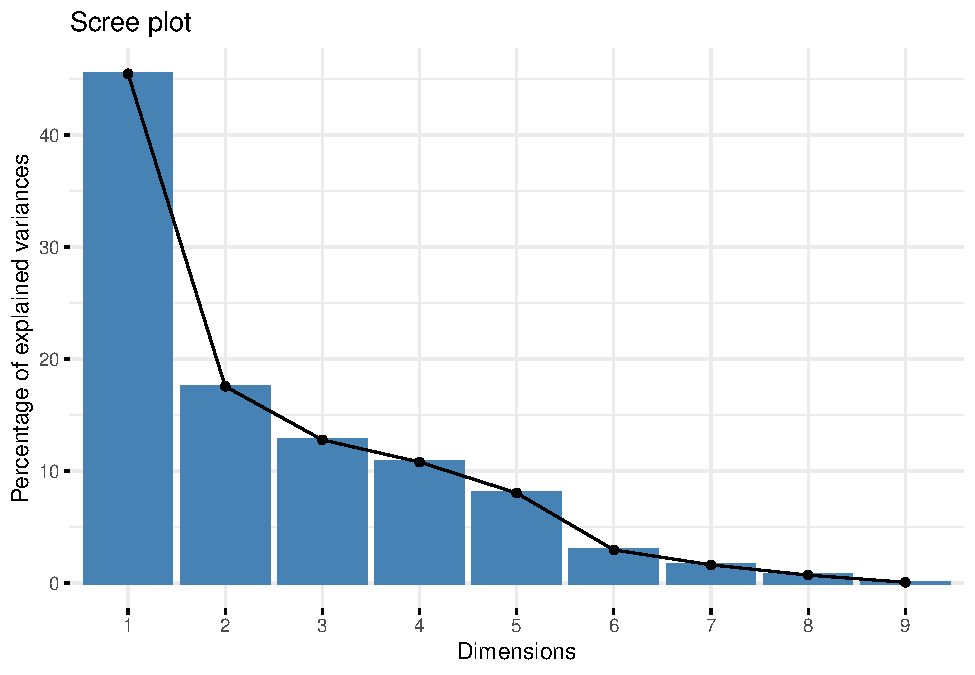
\includegraphics{Rapport_Final_files/figure-latex/unnamed-chunk-3-1} 

}

\caption{\label{fig:arbre} Arbre optimal utilisant un cp de `r format(choixCP, digits=5, scientific =FALSE)`, un minbucket de `r choixMinbucket` et l'indice de Gini comme fonction de perte.}\label{fig:unnamed-chunk-3}
\end{figure}

\newpage

\subsection{Un ensemble d'arbres de décision agrégées par
bagging}\label{un-ensemble-darbres-de-duxe9cision-agruxe9guxe9es-par-bagging}

Le modèle d'ensemble d'arbres de décision agrégée par bagging permet
d'obtenir des prévisions à partir d'un nombre d'arbres de décision,
chacun ajusté par un échantillon bootstrap de l'échantillon
d'entrainement. Une prévision du bagging correspondra à la classe
prédite majoritaire (renouvellement ou résignation) par les arbres de
classifications puisqu'il s'agit d'un problème de classification. Chacun
des arbres utilise l' \emph{indice de Gini} comme fonction de perte.
Nous avons fait ce choix puisqu'à la section précédente portant sur
l'arbre de classification, on a pu démontrer que l' \emph{indice de
Gini} était préférable à l'entropie croisée pour notre jeu de donnée.

Avant l'optimisation d'hyperparamètre, il est nécessaire de déterminer
un nombre d'arbres suffisant pour améliorer les prévisions. Pour ce
faire, nous ajustons un modèle bagging avec un nombre d'arbres plus
élevé que nécessaire avec l'échantillon d'entrainement. Ce modèle
bagging de base n'a pas de pas de contrainte appliquée sur chacun des
arbres puisque ce sera optimisé par la suite. Pour déterminer le nombre
d'arbres adéquat, nous avons tracé un graphique du taux d'erreur
\emph{OOB} en fonction du nombre d'arbres \emph{T}.

\begin{figure}

{\centering \includegraphics{Rapport_Final_files/figure-latex/plot_OOB_bagging-1} 

}

\caption{Taux d'erreur OOB en fonction du nombre d'arbre B}\label{fig:plot_OOB_bagging}
\end{figure}

Comme on peut le voir dans le graphique, le taux d'erreur \emph{OOB} se
stabilise à partir d'un nombre d'arbres de 100 et plus. Le nombre
d'arbres de notre bagging sera donc de 100.

\newpage

L'hyperparamètre qui sera optimisé par la suite pour augmenter les
performances du bagging est le paramètre de la taille minimale d'un
noeud (nodesize) pour chacun des arbres du modèle bagging. Des tailles
de noeuds minimales partant de 2 allant jusqu'à 40 seront testées. Pour
l'optimisation, on s'intéressera à maximiser la métrique AUC. Pour
chaque taille de noeud, un AUC moyen sera calculé à partir d'une
validation croisée par 4 ensembles. Voici les résultats obtenus de la
validation croisée.

\begin{center}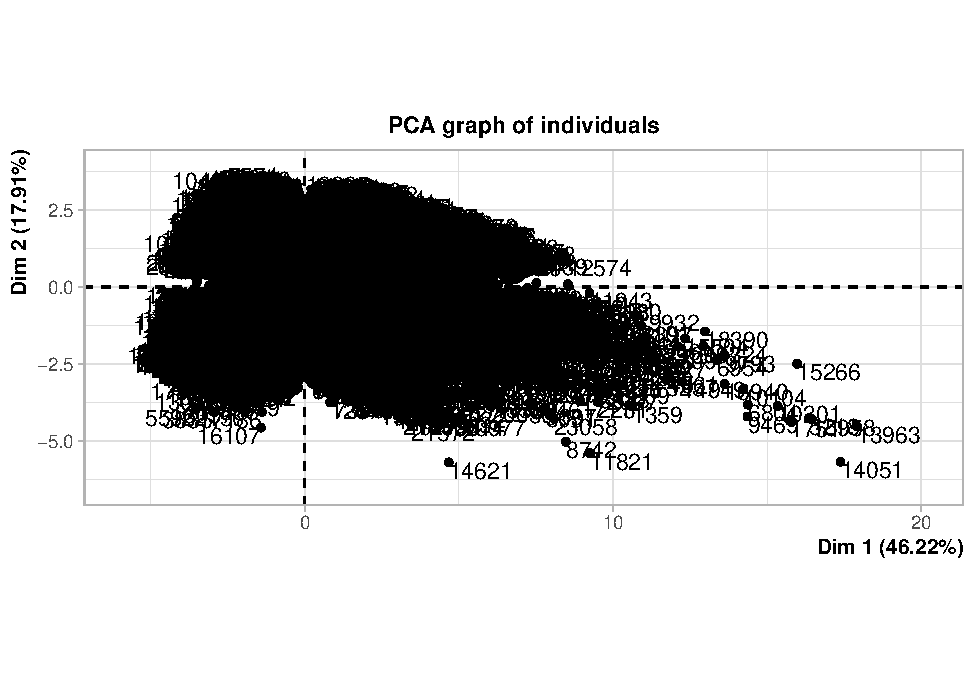
\includegraphics{Rapport_Final_files/figure-latex/unnamed-chunk-4-1} \end{center}

On constate que l'AUC est maximisé lorsque \emph{nodesize} prend une
valeur de 34. Le modèle d'ensemble d'arbres de décision agrégée par
bagging choisi aura donc un nombre d'arbres de 100 et une taille
minimale d'un noeud pour les arbres de 34.

\newpage

\subsection{Forêt aléatoire}\label{foruxeat-aluxe9atoire}

La forêt aléatoire permet elle aussi d'obtenir des prévisions à partir
de prévisions agrégées d'arbre de classification. La fonction de perte
utilisée à chaque arbre est encore l' \emph{indice de Gini} pour la même
raison mentionnée précédemment. Cependant, un changement par rapport au
bagging est la taille de l'échantillon boostrap pour ajuster les arbres.
Puisque notre jeu de données est assez volumineux et que cette fois-ci,
nous devrons optimiser deux hyperparamètres plutôt qu'un, nous avons
choisi de prendre une taille d'échantillon bootsrap correspondant à 50\%
de l'échantillon d'entraînement pour réduire les temps de calcul de
l'optimisation.

Avant de procéder à l'optimisation, il est encore nécessaire de
déterminer un nombre d'arbres suffisant pour la forêt. Pour ce faire,
nous avons ajusté un modèle de forêt classique avec un nombre d'arbres
plus élevé que nécessaire. Comme pour le bagging, pour déterminer le
nombre d'arbres adéquat, nous avons tracé un graphique du taux d'erreur
\emph{OOB} en fonction du nombre d'arbres \emph{T}.

\begin{figure}

{\centering \includegraphics{Rapport_Final_files/figure-latex/plot_OOB_forest-1} 

}

\caption{Taux d'erreur OOB en fonction du nombre d'arbre B}\label{fig:plot_OOB_forest}
\end{figure}

\newpage

Comme on peut le voir dans le graphique, le taux d'erreur \emph{OOB} se
stabilise à partir d'un nombre d'arbres de 100 et plus comme le bagging.
Le nombre d'arbres de notre forêt aléatoire sera donc de 100. Il y a
deux hyperparamètres qui seront optimisés soient la taille minimale d'un
noeud (nodesize) et le nombre de prédicteurs choisi de façon aléatoire
(mtry) à chaque noeud de la forêt aléatoire. Pour chaque \emph{nodesize}
allant de 5 jusqu'à 40 par multiple de 5, un \emph{mtry} optimal est
obtenu par validation croisée à 5 plis. La métrique d'intérêt de
l'optimisation est l' \emph{AUC}. Ce sont donc, des couples optimaux qui
sont obtenus. Voici les résultats obtenus.

\begin{table}[!ht]
\centering
\begin{tabular}{ccc}
\hline
\multicolumn{3}{c}{} \\
nodesize & mtry & AUC \\ 
  \hline
5 & 4 & 0.5966 \\ 
  10 & 5 & 0.5992 \\ 
  15 & 6 & 0.6015 \\ 
   \hline
20 & 10 & 0.6053 \\ 
   \hline
25 & 14 & 0.5969 \\ 
  30 & 8 & 0.5921 \\ 
  35 & 10 & 0.5940 \\ 
  40 & 8 & 0.5911 \\ 
   \hline
\end{tabular}
\end{table}

On constate que le couple d'hyperparamètres qui a obtenu l' \emph{AUC}
le plus élevé correspond à un \emph{nodesize} de 20 et un \emph{mtry} de
10. En somme, la forêt aléatoire choisie aura donc les caractéristiques
suivantes:

\begin{itemize}
\item La taille d'échantillon boostrap est de 50\% de l'échantillon d'entrainement
\item La forêt aléatoire est composée de 100 arbres 
\item La taille minimale d'un noeud (nodesize) d'un arbre est de 20 observations
\item Le nombre de prédicteurs choisis de façon aléatoire (mtry) à chaque embranchement est de 10
\end{itemize}

\newpage

\subsection{Boosting de gradient
stochastique}\label{boosting-de-gradient-stochastique}

Le modèle de boosting de gradient est un modèle de boosting généralisé
pour toute fonction de perte d'intérêt. Dans notre cas, nous utiliserons
le boosting de gradient dans un cas de classification. Ainsi, la
fonction de perte d'intérêt est la \emph{déviance de la loi Bernoulli}.
À ces fins, les données ont dû être temporairement transformées en
données booléennes de type 0 et 1 pour l'élaboration du modèle.

Il est à noter que l'idée générale est d'améliorer la prévision le plus
possible à l'itération \emph{t} en trouvant un arbre
\(\widehat{f}_{\text{arbre}}^t\) afin de minimiser la perte

\begin{align}
   \sum_{i=1}^n \mathcal{L} \left\{ y_i, \widehat{f}_{t-1}(x_i) + \widehat{f}_{\text{arbre}}^t(x_i) \right\}.
\end{align}

La perte se retrouve minimisée, car à chaque itération, un pas de plus
est effectué dans la direction du gradient négatif. De plus, étant donné
qu'on utilise la déviance négative d'une loi bernouilli comme fonction
de perte,

\begin{align}
    \mathcal{L} = \sum_{k=1}^2 \widehat{P}_{ik} \ln( \widehat{P}_{ik}).
\end{align}

Ce modèle choisit un sous-échantillon de taille inférieur à \(n\) pour
ajuster l'arbre au lieu d'utiliser un échantillon de taille similaire à
l'échantillon d'entrainement à chaque fois. Cette manière de procéder
permet de réduire le temps d'entrainement et peut améliorer la précision
des prévisions étant donné que ce ne sera pas toujours les mêmes données
qui risquent de se retrouver dans chacun des arbres.

La procédure d'optimisation des hyperparamètres a été effectuée pour la
fonction de perte visée. Les hyperparamètres sont \textbf{n.trees},
\textbf{interaction.depth}, \textbf{shrinkage} et
\textbf{n.minobsinnode} représentant respectivement le nombre d'arbres
dans le boosting, la profondeur maximale de l'arbre, le taux
d'apprentissage \(\lambda\) et le nombre d'observations minimal par
noeud. On optimisera seulement \textbf{n.trees} et
\textbf{interaction.depth}, car les deux autres hyperparamètres peuvent
être choisis facilement dans le but d'avoir un temps d'exécution
raisonnable. Selon les tests effectués au préalable on prendra un
\(\lambda = 0.005\) et un \(n.minobsinnode = 20\).

L'optimisation des deux hyperparamètres restants est ensuite faite à
partir de la validation croisée sur 4 ensembles. C'est une méthode
d'optimisation qui permet de trouver les hyperparamètres optimaux sur
chacun des plis pour ensuite choisir les hyperparamètres optimaux sur
l'ensemble des données d'entrainement. Le choix se fera à l'aide de la
métrique \emph{ROC}. Le choix des paramètres est donc effectué selon
l'aire sour la courbe ROC ( \emph{AUC}) obtenue la plus élevée. On
observe ainsi aisément à l'aide de la \autoref{fig:gbm.plotoptimisation}
que le modèle choisit utilisera un \(n.trees(T) =\) 2100, un
\(interaction.depth(d) =\) 3 et comme indiqué précédemment, un
\(shrinkage(\lambda) = 0.005\), un \(n.minobsinnode = 20\) et la
déviance négative d'une loi bernoulli comme fonction de perte. C'est
avec ces valeurs que le modèle atteint la plus haute performance pour un
temps de calcul raisonnable. Le graphique nous indique bien le choix des
valeurs, car on choisit ce qui permet au modèle d'atteindre la plus
haute valeur pour l' \emph{AUC}. Il est à noter que pour une meilleure
performance le taux d'apprentissage aurait été plus faible et le nombre
d'arbres plus élevé ce qui demande une espace de stockage et un temps de
calcul beaucoup plus important.

\newpage

\begin{figure}

{\centering \includegraphics{Rapport_Final_files/figure-latex/gbm.plotoptimisation-1} 

}

\caption{Résultats obtenu pour l'optimisation des paramètres à partir de la fonction train en R.}\label{fig:gbm.plotoptimisation}
\end{figure}

\newpage

\section{Comparaison des modèles}\label{comparaison-des-moduxe8les}

Dans cette section, il sera question de comparer la performance
prédictive des différents modèles. Pour ce faire, nous analyserons la
performance de la prévision sur les données tests à l'aide de la courbe
ROC et de la valeur de l'AUC, soit l'aire sous la courbe ROC.

Les modèles ayant l'AUC la plus élevée sont les modèles ayant la
performance de prévision la plus élevée basée sur cette métrique. La
\autoref{fig:plot_ROC} illustre les différentes courbes ROC obtenu pour
les différents modèles et le \autoref{tbl:tableau-AUC} présente les
valeurs d'AUC qui découle de ces courbes.

\begin{table}[ht]
\centering
\caption{Aire sous la courbe ROC pour chacun des différents modèles} 
\label{tbl:tableau-AUC}
\begin{tabular}{lr}
  \hline
Modèles & AUC \\ 
  \hline
Modèle de base GLM & 0.625 \\ 
  Modèle linéaire avec régularisation Lasso & 0.552 \\ 
  modèle des k plus proches voisins & 0.574 \\ 
  Arbre de décision & 0.597 \\ 
  Ensemble d'arbres de décision agrégées par bagging & 0.589 \\ 
  forêt aléatoire & 0.594 \\ 
  Modèle de gradient boosting & 0.632 \\ 
   \hline
\end{tabular}
\end{table}

\begin{figure}

{\centering \includegraphics{Rapport_Final_files/figure-latex/plot_ROC-1} 

}

\caption{Courbe ROC pour chacun des différents modèles}\label{fig:plot_ROC}
\end{figure}

La courbe ROC est définie comme étant la sensitivité en fonction du faux
négatif. Dans le but d'avoir une bonne performance prédictive, on
cherche à maximiser la sensitivité et la spécificité, ce qui se traduit
en une courbe se rapprochant le plus possible du coin supérieur gauche.
En ayant utilisé cette métrique pour classifier la performance, on peut
baser notre choix sur les modèles ayant l'AUC le plus élevée. Les deux
modèles les plus performants sont le modèle de base GLM et le modèle de
boosting de gradient stochastique. La suite de l'analyse sera donc
spécifique à ces deux modèles. Malgré le fait que ces modèles soient les
plus performant sur nos données, il est décevant de voir que nous sommes
en mesure d'atteindre seulement 63\% d'AUC.

\newpage

\section{Interprétation des meilleurs
modèles}\label{interpruxe9tation-des-meilleurs-moduxe8les}

Dans cette section, on interprète le modèle de base, soit le modèle
linéaire généralisé, et le modèle de gradient stochastique, car ce sont
ceux ayant la meilleure performance sous la mesure \emph{AUC} de la
qualité de l'ajustement. Les méthodes utilisées pour l'interprétation
diffèreront entre autres, car le modèle de boosting de gradient
stochastique est construit sur un nombre élevé d'arbres. Pour avoir
l'effet spécifique de chacune des variables sur la prévision, il
faudrait analyser chacun des arbres individuellement, ce qui n'est
évidemment pas optimal. On aura recourt à des outils permettant de
visualiser l'impact global de chacune des variables sur l'ensemble des
arbres, ce qui est un peu moins précis que pour le modèle de base. Le
GLM permet d'avoir un facteur associé à chacune des variables
directement. Ces facteurs sont une mesure directe de l'impact des
variables sur la prévision. Ainsi, on tente d'avoir une mesure semblable
pour le modèle de boosting de gradient nous permettant de visualiser
l'impact des variables sur la prévision sans avoir à passer en revue
chacun des arbres entrainés.

\subsection{Modèle de base}\label{moduxe8le-de-base-1}

Comme mentionné précédemment, l'interprétation de ce modèle se fera sur
les valeurs que prend les coefficients, soit les valeurs des \(\beta_i\)
qui multiplie chacune des variables dans l'équation. Étant donné qu'on
modélise la probabilité de non-renouvellement des assurés de cette
compagnie d'assurance, le lien logistique a été utilisé dans
l'élaboration du modèle. En isolant, on peut obtenir l'équation suivante
:

\[\eta = ln\left(\frac{\pi_{res}}{1 - \pi_{res}}\right) \quad \Leftrightarrow \quad \pi_{res} = \frac{e^{\eta}}{1 + e^{\eta}} \text{(fn expit)}.\]

Il est à noter que \(\pi_{res}\) représente la probabilité de
résignation de l'assuré pour lequel on veut obtenir une prévision.
L'interprétation qui en ressort est que lorsque la probabilité de
résignation est croissante lorsque le prédicteur linéaire \(\eta\)
augmente et décroissante lorsque que \(\eta\) est décroissant. Le
prédicteur linéaire est défini comme

\[\eta = \sum\limits_{j=1}^p \beta_{j} x_{j}.\]

Un coefficient négatif indique que la probabilité de résignation de la
police d'assurance diminue et inversement, lorsque le coefficient est
positif, la probabilité de résignation augmente. Sachant que le modèle
comprend un grand nombre de variables explicatives, un tableau résumé
(voir \autoref{tbl:glm_coeff}) a été conçu et ajouté à ce rapport dans
le but de synthétiser l'interprétation qu'on peut en faire. Le
coefficient d'origine aura un impact négatif sur la prévision.
\textbf{C'est-à-dire que la prévision part avec une probabilité de
résignation qui diminue}. De plus, selon l'équation du modèle plus la
valeur d'une variable numérique est élevée, plus l'impact sur la
prévision sera remarquable sur la prévision.

On interprète ensuite le tableau comme suit :

\begin{itemize}
\item
  Les variables \emph{polholder\_age}, \emph{policy\_age},
  \emph{prem\_last}, \emph{prem\_market} et \emph{vehicl\_age} feront
  baisser la probabilité de résignation. Ainsi, plus l'âge de l'assuré,
  l'âge du véhicule et l'âge de la police augmente et plus la
  probabilité de non-renouvellement diminue. De plus, plus la prime du
  marché augmente plus les assurés seront tenté de garder leur police
  d'assurance, car ils n'auront pas intérêt à s'assurer ailleurs à un
  prix qui vient tout juste d'augmenter ;
\item
  \emph{prem\_final} : l'augmentation de la prime proposée pour le
  renouvellement de la police fait augmenter la probabilité de
  résignation, ce qui fait beaucoup de sens;
\item
  \emph{polholder\_diffdriver} : Une police ayant un conducteur de 24
  ans et plus n'aura aucun impact sur la probabilité. La probabilité de
  résignation sera par contre plus élevée si le conducteur est un
  apprenti, un partenaire ou un jeune, tandis que la probabilité sera
  plus faible lorsque le conducteur est un utilisateur commercial ou un
  utilisateur seul;
\item
  \emph{Polholder\_age} : Le sexe de l'assuré n'aura aucun impact sur la
  probabilité lorsque l'assurée est une femme tandis que lorsque
  l'assuré est un homme, la probabilité de résignation aura tendance à
  augmenter;
\item
  \emph{polholder\_BMCevol} : La probabilité de résignation reste neutre
  lorsque la prime a baissé depuis le dernier renouvellement. L'impact
  sur la prévision sera cependant négatif lorsque la prime a augmenté ou
  est restée stable depuis le dernier renouvellement;
\item
  \emph{polholder\_job} : L'emploi de l'assuré n'aura aucun impact sur
  la prévision si l'assuré travaille dans le domaine médical. Dans tout
  autre domaine, la prévision aura tendance augmenter et donc l'assuré
  sera plus prompt à résigner sa police d'assurance;
\item
  \emph{vehicl\_region} : Ne sachant pas le nom des régions des assurés,
  il est impossible de ressortir une cause possible, mais la région de
  l'assuré n'aura aucun effet sur la prévision lorsqu'elle est de 1.
  L'effet sera négatif pour les régions 2, 5 et 7 et positif pour toutes
  les autres régions;
\item
  \emph{prem\_freqperyear} : pour ce qui est de cette variable, une
  fréquence de paiement choisie à une fois par année n'aura aucun impact
  sur la probabilité de résigner. Les assurés faisant des paiements
  semestriels auront une probabilité moins élevée de résigner leur
  police et comparativement à ceux faisant leur paiement
  semestriellement ou mensuellement qui auront une probabilité plus
  élevée.
\end{itemize}

\begin{table}[ht]
\centering
\caption{Signe des coefficients du GLM} 
\label{tbl:glm_coeff}
\begin{tabular}{lccr}
  \hline
Coefficients & Positif & Negatif & Niveau.neutre \\ 
  \hline
Intercept &  & x & - \\ 
  polholder age &  & x & - \\ 
  polholder BMCevol (inchangée, hausse) &  & x & baisse \\ 
  polholder diffdriver (apprenti, partenaire, jeune) & x &  & 24 ans et plus \\ 
  polholder diffdriver (commerciale, utilisateur seul) &  & x & 24 ans et plus \\ 
  polholder gender (Male) & x &  & Female \\ 
  polholder job (normal) & x &  & medical \\ 
  policy age &  & x & - \\ 
  prem final & x &  & - \\ 
  prem freqyear (2) &  & x & 1 \\ 
  prem freqyear (4, 12) & x &  & 1 \\ 
  prem last &  & x & - \\ 
  prem market &  & x & - \\ 
  vehicl age &  & x & - \\ 
  vehicl region (3, 4, 6, 8 à 14) & x &  & 1 \\ 
  vehicl region (2, 5, 7) &  & x & 1 \\ 
   \hline
\end{tabular}
\end{table}

Étant donné le grand nombre de variables ayant un impact sur la
prévision, on a cru bon d'intégrer à l'interprétation un tableau
sommatif des variables ayant le plus grand impact sur la prévision (voir
\autoref{tbl:betas}). De ce tableau, on peut voir que ces variables sont
\emph{polholder\_BMCevol}, \emph{polholder\_diffdriver} et
\emph{vehicl\_region}. Plus particulièrement, on parle des polices ayant
connu une hausse dans le montant de la prime depuis le dernier
renouvellement, les conducteurs utilisant leur véhicule pour une raison
commerciale et les polices ayant de jeunes conducteurs inscrits, les
assurés effectuant leur paiement semestriellement et les assurés vivant
dans les régions 2, 12, 13 et 14. Les polices ayant des caractéristiques
faisant partie de celles nommées précédemment et figurant dans la
\autoref{tbl:betas} sont donc ceux ayant une probabilité de résignation
plus susceptible de varier.

\begin{table}[ht]
\centering
\caption{Valeurs des coefficients ayant le plus grand impact sur la prévision.} 
\label{tbl:betas}
\begin{tabular}{lr}
  \hline
variables & coefficients \\ 
  \hline
Intercept & -1.1852 \\ 
  polholder BMCevol (stable) & -0.4392 \\ 
  polholder BMCevol (hausse) & -0.714 \\ 
  polholder diffdriver (commerciale) & -0.7417 \\ 
  polholder diffdriver (apprenti) & 0.663 \\ 
  polholder diffdriver(jeune) & 0.3618 \\ 
  prem freqperyear(2) & -0.4298 \\ 
  vehicl region (2) & -0.4764 \\ 
  vehicl region (12) & 0.6005 \\ 
  vehicl region (13) & 0.3543 \\ 
  vehicl region (14) & 0.3783 \\ 
   \hline
\end{tabular}
\end{table}

\newpage

\subsection{Boosting de gradient
stochastique}\label{boosting-de-gradient-stochastique-1}

L'interprétation de ce modèle étant plus demandante que pour le modèle
de base étant donné le nombre élevé d'arbres entraînés, certains outils
devront être utilisés. Ces outils sont l'importance des variables, les
graphiques de dépendance partielle et la statistique H de Friedman.

L'importance des variables nous permet de comprendre l'influence des
variables explicatives sur la prévision. Ainsi, on peut visualiser les
variables du modèle ayant le plus grand impact sur la prévision. De la
\autoref{fig:imp-gbm}, on voit que les variables les plus significatives
sur ce modèle sont définitivement \emph{prem\_index} et
\emph{vehicl\_region}, tout comme \emph{prem\_freqperyear},
\emph{polholder\_age} et \emph{vehicl\_age} et d'autres, mais qui ont
une mesure d'importance moins considérable que les deux premières. Les
valeurs sur lesquelles on se fie pour tirer cette conclusion viennent de
l'importance relative des variables prises individuellement sur la
prévision. Plus cette valeur est élevée, plus la valeur de la variable a
un impact non négligeable sur la prévision. Dans le but de mieux
comprendre l'effet individuel des variables ayant le plus grand impact,
on utilisera l'outil des graphiques de dépendances partielles en se
concentrant sur les variables \emph{prem\_index} et
\emph{vehicl\_region}.

\begin{figure}
\centering
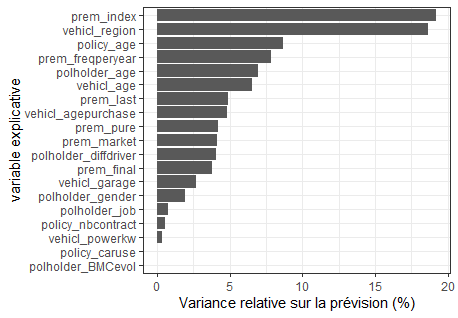
\includegraphics{../src/07-gbm/imp_gbm}
\caption{Graphique de l'importance des variables sur la prévision}
\label{fig:imp-gbm}
\end{figure}

Ces graphiques permettent une interprétation plus spécifique. Étant
donné que l'importance des variables ne nous permet pas de comprendre
l'effet isolé d'une variable explicative sur la prévision, c'est à
l'aide de cet outil qu'on pourra en faire l'interprétation. Il est ainsi
utilisé pour mieux comprendre l'effet global d'une variable explicative
sur la prévision et peut être interprété comme la moyenne des ICEs, soit
l'espérance conditionnelle individuelle pour chacune des observations.

Le graphique de gauche de la \autoref{tbl:pdppartie1} nous permet de
voir que pour une valeur de \emph{prem\_index} se situant entre 0 et
0.6, la probabilité de résignation est beaucoup plus faible. Ainsi, un
assuré peut avoir un pourcentage d'augmentation de sa prime au
renouvellement allant jusqu'à presque 50\% sans qu'il y ait
nécessairement un impact sur sa probabilité de résigner. C'est lorsque
l'augmentation dépasse les 55\% environ qu'on remarque l'impact de
l'augmentation de la prime sur la probabilité de résigner. Il est
surprenant de voir que lorsque qu'il y a une petit diminution de prime,
la probabilité augmente de beaucoup. Cette effect est difficilement
expliquable sans l'aide de d'autres variables explicatives.

Le graphique de droite de la \autoref{tbl:pdppartie1} nous permet, quant
à elle, de voir que les régions 11 à 14 sont celles affectant le plus la
probabilité de ne pas renouveler la police d'assurance. L'impact le plus
marqué est observé auprès des assurés ayant comme région de résidence la
région 12 et l'impact le moins marqué est observé auprès des résidents
de la région 2. Étant donné que les noms des régions n'ont pas été
divulgués par la compagnie d'où provient le jeu de données, il est
impossible pour nous de faire un lien entre la région et l'impact que
celle-ci peut avoir sur la décision de l'assuré qui y habite.

\begin{figure}
\centering
\begin{minipage}{0.48\linewidth}

\begin{center}\includegraphics{Rapport_Final_files/figure-latex/pdp_prem_index-1} \end{center}
\end{minipage}
\hfill
\begin{minipage}{0.48\linewidth}

\begin{center}\includegraphics{Rapport_Final_files/figure-latex/pdp_vehicl_region-1} \end{center}
\end{minipage}
\caption{Graphique de dépendance partielle pour les variables prem.index et vehicl.region.}
\label{tbl:pdppartie1}
\end{figure}

\begin{figure}
\centering
\begin{minipage}{0.48\linewidth}

\begin{center}\includegraphics{Rapport_Final_files/figure-latex/pdp_prem_policy_age-1} \end{center}
\end{minipage}
\hfill
\begin{minipage}{0.48\linewidth}

\begin{center}\includegraphics{Rapport_Final_files/figure-latex/pdp_prem_freqperyear-1} \end{center}
\end{minipage}
\caption{Graphique de dépendance partielle pour les variables policy.age et prem.freqperyear.}
\label{tbl:pdppartie2}
\end{figure}

De plus, en jetant un coup d'oeil aux autres variables ayant une
importance marquée sur la prévision, il a été possible d'observer un
effet important de l'âge de la police et de la fréquance de paiement de
la prime sur la probabilité de résignation d'où l'ajout de la
\autoref{tbl:pdppartie2} à ce rapport. Dans celles-ci, on peut observer
que la probabilité de résignation diminue avec l'âge de la police, ce
qui montre une certaine forme de fidélité des clients. De plus dès que
la police atteint plus de 5 ans, cette probabilité reste stable à une
valeur qui s'approche grandement de la valeur nulle. Dans le cas de la
variable \emph{prem\_freqperyear}, on observe que plus la fréquence de
paiement est élevé, plus la probabilité de résignation diminue.

\newpage

Pour ce qui est de la statistique H de Friedman, elle est utilisée pour
pouvoir estimer la force des interactions entre une variable précisément
et tous les autres variables en mesurant la quantité de la variance qui
provient de cette interaction dans la prévision. On peut ainsi observer
les variables qui interagissent avec les variables les plus importantes
pour expliquer la prévision, soit les variables \emph{prem\_index} et
\emph{vehicl\_region}. Sachant que la profondeur maximale de l'arbre
pour ce modèle est de 3, il pourrait y avoir des interactions sur
jusqu'à 3 variables différentes. Par cette statistique, on obtient les
graphiques suivants.

\begin{figure}

{\centering \includegraphics{Rapport_Final_files/figure-latex/int_prem_index-1} 

}

\caption{\label{int}Graphique de l'importance des interractions entre la variables prem.index et les autres variables sur la prévision}\label{fig:int_prem_index}
\end{figure}

La \autoref{int} est un exemple de graphique obtenu en utilisant cette
statistique. On peut ensuite utiliser les graphiques de dépendance
partielle pour voir l'impact des interactions ayant la plus grande force
sur la prévision. Après analyse, seule l'interaction
\emph{vehicl\_region:prem\_index} donne une interprétation intéressante.
À partir de graphique de dépendance partielle de la \autoref{pdp}, on
peut observer que certaines régions possèdent un creux où la probabilité
de résignation est beaucoup plus faible lorsque le pourcentage
d'augmentation de la prime ce situe entre 0 et 50\% dont les régions 1,
2, 8, 9, 12, 13 et 14. Pour ce qui est des autres régions, la
probabilité de résignation demeure assez stable et faible lorsque le
pourcentage d'augmentation est supérieur à 0\%.

\begin{figure}

{\centering \includegraphics{Rapport_Final_files/figure-latex/dpd_interraction-1} 

}

\caption{\label{pdp}Graphique de dépendance partielle pour l'interraction entre la variable vehicl.region et la variable prem.index}\label{fig:dpd_interraction}
\end{figure}

\subsubsection{Prédiction sur les données
tests}\label{pruxe9diction-sur-les-donnuxe9es-tests}

Puisque nous avons choisit l'AUC comme métrique de sélection, il est
difficile de dire comment le modèles prédit exactement les données.
C'est pourquoi la autoref\{tbl:conf-matrice-modele-final\} montre les
résultats des prédictions sur les données tests en utilisant le seuil
optimal qui mène au point le plus proche du coin haut gauche de la
courbe ROC. On remarque que le modèle gbm prédit mieux les vrai
renouvellement et moins de faux renouvellement que le glm. En
opposition, le glm prédit légérement mieux les vrais résignations et
prédit moins de fausse résignation.

\begin{table}[!ht]
\centering
\caption{Tableau de confusion en utilisant le seuil optimal pour les deux 
meilleurs modèles sélectionnés.}
\label{tbl:conf-matrice-modele-final}
\begin{minipage}{0.48\linewidth}
\begin{tabular}{l|cc}
\multicolumn{1}{c}{} & \multicolumn{2}{c}{Prédiction} \\
GLM & Renouvellement & Résignation \\
\hline
Renouvellement & 2317 & 1704 \\
Résignation    & 233 & 357 \\
\hline
\end{tabular}
\end{minipage}
\hfill
\begin{minipage}{0.48\linewidth}
\begin{tabular}{l|cc}
\multicolumn{1}{c}{} & \multicolumn{2}{c}{Prédiction} \\
GBM & Renouvellement & Résignation \\
\hline
Renouvellement & 2509 & 1512 \\
Résignation    & 262 & 328 \\
\hline
\end{tabular}
\end{minipage}
\end{table}

\newpage

\section{Conclusion}\label{conclusion}

En vu des des tableaux de confusion de la section précédante, le modèles
qui devrait être utilisé par la compagnie d'assurance pour prédire les
résignations serait le modèle GBM pour deux raisons.

Premièrement, comme discuté précédament, chaque matrice de confusion
offre des avantages et des désavantage, mais les avantages sont
meilleurs pour le gbm. Par exemple, on augmente de 192 les vrai
renouvellement pour seulement augmenter de 29 les faux renouvellement.

Deuxièmement, prenon le cas ou la prédiction servirait à optimisé la
statégie de renouvellement des assurés, par exemple en augmentant plus
les assurées avec un faible probabilité de résignation. Dans ce cas, le
fait de prédire des faux renouvellement n'a aucun effet puisque peut
importe l'augmentation, l'assuré aurait résigné; conséquament, ceci n'a
pas d'impact sur la rentabilité. Ainsi, la matrice de confusion qui
maximise les vrai renouvellement au coût de prédire plus de faux
renouvellement est le modèle gbm.

Finalement, bien que le modèle final soit le gradient boosting, les
résultats auraient pu être meilleurs. En effet, beaucoup de faux
renouvellement sont généré ce qui pourrait avoir des effets sur la
rentabilité de la compagnie puisqu'elle aurait pu charché plus cher à
ceux-ci. Le modèle pourrait être amélioré est utilisant des méthodes
pour contourné le problème de débalancement des données, par exemple en
utilisant des techniques de sous et sur échantillionnage. Il aurait
aussi été intéréssant d'avoir plus d'information sur l'expérience des
assurés autre que le système Bonus Malus. Par exemple, la fréquence
d'accident ainsi que le coût de ses accident. De plus, nous avons vu que
la régions avait un impact important. Il aurait été pertinant de savoir
en quoi consiste ses différentes régions.

\newpage

\section*{Bibliographie}\label{bibliographie}
\addcontentsline{toc}{section}{Bibliographie}

\hypertarget{refs}{}
\hypertarget{ref-AnalyseComposantesPrincipales}{}
Côté, Marie-Pier. 2020a. \emph{ACT-3114 - Analyse En Composantes
Principales}. Recueil inédit; Université Laval.

\hypertarget{ref-Arbre}{}
---------. 2020b. \emph{ACT-3114 - Arbres de Classification et de
Régrssion}. Recueil inédit; Université Laval.

\hypertarget{ref-baggingEtForet}{}
---------. 2020c. \emph{ACT-3114 - Bagging et Forêts Aléatoires}.
Recueil inédit; Université Laval.

\hypertarget{ref-Boosting}{}
---------. 2020d. \emph{ACT-3114 - Boosting, Adaboost et Boosting de
Gradient Stochastique}. Recueil inédit; Université Laval.

\hypertarget{ref-ClassificationNonSupervisuxe9e}{}
---------. 2020e. \emph{ACT-3114 - Classification Non-Supervisée}.
Recueil inédit; Université Laval.

\hypertarget{ref-Communication}{}
---------. 2020f. \emph{ACT-3114 - Communication et Interprétation}.
Recueil inédit; Université Laval.

\hypertarget{ref-IntroAppSupervise}{}
---------. 2020g. \emph{ACT-3114 - Introduction à L'apprentissage
Supervisé}. Recueil inédit; Université Laval.

\hypertarget{ref-TraitementDonnesManquantes}{}
---------. 2020h. \emph{ACT-3114 - Traitement Des Données Manquantes}.
Recueil inédit; Université Laval.

\hypertarget{ref-VisualisationPretraitement}{}
---------. 2020i. \emph{ACT-3114 - Visualisation et Prétraitement}.
Recueil inédit; Université Laval.

\hypertarget{ref-CASdatasets}{}
Dutang, Christophe, and Arthur Charpentier. 2019. \emph{CASdatasets:
Insurance Datasets}. R Package Version 1.0-10.
\url{http://cas.uqam.ca/}.

\hypertarget{ref-glmnet.intro}{}
Hastie, Trevor, and Junyang Qian. 2016. \emph{An Introduction to
Glmnet}.
\url{https://cran.r-project.org/web/packages/glmnet/vignettes/glmnet.pdf}.

\hypertarget{ref-Caret}{}
Kuhn, Max. 2020. \emph{Caret: Classification and Regression Training}. R
Package Version 6.0-86. \url{https://CRAN.R-project.org/package=caret}.

\end{document}
